\section{物质的结晶}\label{sec:4-4}

\subsection{结晶}

把固体溶质的水溶液放在敞口的容器里,让水慢慢地蒸发,溶液达到饱和以后,如果继续蒸发,
过剩的溶质就能成固体析出( 图 \ref{fig:4-5})。
对溶解度受温度变化的影响不大的固体溶质,一般就用这种蒸发溶剂的方法得到固体。
例如,从海水提取食盐,就是把海水引到盐滩上,利用日光和风力使水分蒸发,得到固体食盐。

对溶解度受温度变化的影响相当大的固体溶质,我们一般用什么方法得到固体呢?

\begin{figure}[htbp]
    \centering
    \begin{minipage}[b]{7cm}
        \centering
        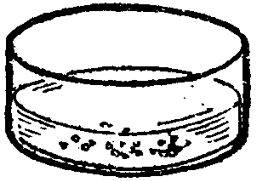
\includegraphics[width=3cm]{../pic/czhx1-ch4-5}
    \caption{溶剂蒸发,溶质从溶液里析出}\label{fig:4-5}
    \end{minipage}
    \qquad
    \begin{minipage}[b]{7cm}
        \centering
        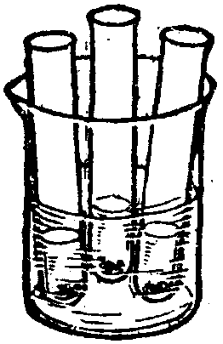
\includegraphics[width=2cm]{../pic/czhx1-ch4-6}
        \caption{饱和溶液冷却,溶质从溶液里析出}\label{fig:4-6}
    \end{minipage}
\end{figure}


\begin{shiyan}\label{shiyan:4-7}
    在 3 个试管里, 各注入 10 毫升蒸馏水。分别在这 3 个试管里加入少量硫酸铜、硝酸钾和明矾,振荡,使它们完全溶解。
    然后给这 3 个试管加热,再继续分别加入硫酸铜、硝酸钾和明矾,制成饱和溶液。
    把盛有饱和溶液的试管,放在冷水中冷却,观察发生的现象(图 \ref{fig:4-6}) 。
\end{shiyan}

饱和溶液冷却后,溶质就从溶液里析出。在这个实验里,用冷却热饱和溶液的方法得到固体。

仔细观察食盐和\nameref{shiyan:4-7}制得的固体,可以看到,这几种固体都具有一定的几何形状。
例如,明矾是八面体,常见的食盐是立方体(图\ref{fig:4-7} 和封里彩图)。

\begin{figure}[htbp]
    \centering
    \begin{minipage}[b]{7cm}
        \centering
        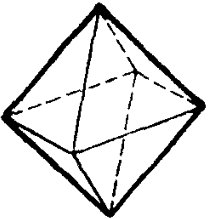
\includegraphics[width=2cm]{../pic/czhx1-ch4-7-1}
    \caption*{明矾}
    \end{minipage}
    \qquad
    \begin{minipage}[b]{7cm}
        \centering
        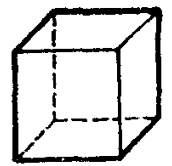
\includegraphics[width=2cm]{../pic/czhx1-ch4-7-2}
        \caption*{食盐}
    \end{minipage}
    \caption{晶体的形状}\label{fig:4-7}
\end{figure}


象上述具有规则的几何外形的固体叫做\zhongdian{晶体}。形成晶体的过程叫做\zhongdian{结晶}。

结晶跟溶解是相反的两个过程。当溶质溶解在溶剂里时,
一方面,溶质的微粒不断地离开溶质表面,扩散到溶剂里去;
另一方面,溶解在溶剂里的溶质微粒不断地在未溶解的溶质表面聚集成为晶体。
所以在溶质进行溶解过程的同时,也在进行结晶的过程,这两个同时进行的相反过程是可逆的,通常用 “\ce{<=>}” 表示。
\begin{fangchengshi}
    \ce{ \text{固体溶质} <=>[\text{溶解}][\text{结晶}] \text{溶液里的溶质} }
\end{fangchengshi}

当溶质开始溶解的时候,在单位时间里,从固体溶质表面扩散到溶剂里的溶质微粒的数目,比回到固体溶质表面的溶质微粒的数目多,
所以,表面看来,固体溶质在不断地溶解(减少)。随着溶液里溶质微粒的逐渐增加,由溶液里回到固体溶质表面的微粒也随之增加,
这时表面看来,溶质溶解的速度逐渐减小,同时溶质结晶的速度就在逐渐增大。直到固体溶质不再溶解时,
即单位时间内扩散到溶液里去的溶质微粒数目,和回到固体溶质表面的溶质微粒的数目相等了,
也就是溶质溶解的速度等于溶质结晶的速度,即达到了平衡。
这时从表面看,溶质不再溶解,也不再结晶,这时的溶液就是我们前面所说的饱和溶液。
这也就是能够溶解在水里的物质,不能无限制地溶解的原因。

为什么冷却上述热饱和溶液能析出溶质的晶体呢?
这是因为,在一定温度下的饱和溶液,溶质溶解的速度等于溶质结晶的速度。
由于这种溶质的溶解度是随着温度的降低而减小的,
当温度降低时,溶质溶解的速度小于溶质结晶的速度,
因此,溶质结晶析出。

\subsection{结晶水和结晶水合物}

许多物质在水溶液里析出,形成晶体时,晶体里常结合一定数目的水分子,这样的水分子叫做\zhongdian{结晶水}。
含有结晶水的物质叫做\zhongdian{结晶水合物}。我们知道某些溶质溶解在水里,
溶质分子(或离子)跟一定数目的水分子结合成为水合物的分子(或水合离子)。
这种水合物有的只能在溶液里存在;有的在结晶的过程中,可以析出成为含结晶水的晶体。

结晶水合物很多,象胆矾(或叫蓝矾 \ce{CuSO4.5H2O})、
石膏(\ce{CaSO4.2H2O})、
绿矾(\ce{FeSO4.7H2O})、
明矾〔\ce{KAl(SO4)2.12H2O}〕等等都是。
有的物质的晶体里不含结晶水,象食盐、硝酸钾的晶体里就不含结晶水。

结晶水合物受热后容易失掉结晶水。

\begin{shiyan}
    取研碎的蓝色硫酸铜晶体 2 - 3 克,放入硬质试管里,照图 \ref{fig:4-8} 所示裝配好。
    慢慢地给试管加热,观察发生的现象。
\end{shiyan}


\begin{figure}[htbp]
    \centering
    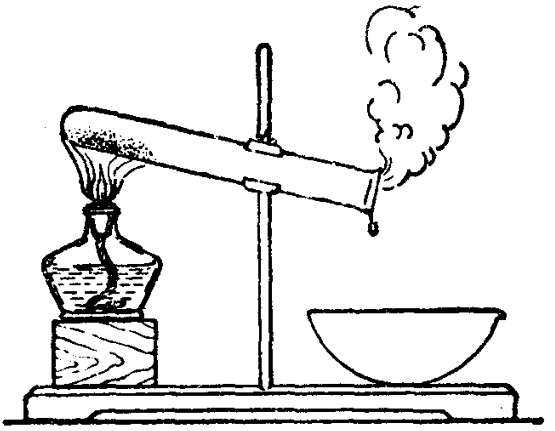
\includegraphics[width=8cm]{../pic/czhx1-ch4-8}
    \caption{给硫酸铜晶体加热}\label{fig:4-8}
\end{figure}



从实验可以看到,蓝色硫酸铜晶体受热后变成了白色粉末,同时,放出水蒸气。
这是因为蓝色硫酸铜晶体受热后失掉了结晶水,生成无水硫酸铜的白色粉末。

经过科学实验测定, 每个 \ce{CuSO4} 跟五个水分子结合在一起,所以,
硫酸铜晶体可用 \ce{CuSO4.5H2O} 表示。上面的化学反应可以表示如下:
\begin{fangchengshi}
    \ce{ \underset{\text{(蓝色)}}{\ce{CuSO4.5H2O}} \xlongequal{\Delta} \underset{\text{(白色)}}{\ce{CuSO4}} + 5H2O ^ }
\end{fangchengshi}


\begin{shiyan}
    往上一实验生成白色硫酸铜粉末的硬质试管里,滴加几滴水,观察颜色的变化。
\end{shiyan}

从实验知道,白色硫酸铜粉末跟水起反应,又重新生成了蓝色硫酸铜晶体。这个化学反应可以表示如下:
\begin{fangchengshi}
    \ce{ \underset{\text{(白色)}}{\ce{CuSO4}} + 5H2O = \underset{\text{(蓝色)}}{\ce{CuSO4.5H2O}} }
\end{fangchengshi}

根据溶解度曲线,能够计算出一定量的一种饱和溶液在温度降低(或溶剂的量减少)的情况下,溶质成为晶体析出的量。

\liti[0] 把 100 克氯化铵的饱和液从 50 ℃ 降低到 10 ℃, 计算有多少克氯化铵析出。

\jie 根据氯化铵的溶解度曲线( 50 ℃ 和 10 ℃ 溶解度分别为 50 克和 33 克),
可算出 150 克氯化铵的饱和溶液从 50 ℃ 降低到 10 ℃ 时有 17 克氯化铵析出。

设 100 克氯化铵的饱和溶液从 50 ℃ 降低到 10 ℃ 析出氯化铵 $x$ 克。
\begin{align*}
    & 150:17 = 100:x \\
    & x = \dfrac{17 \times 100}{150} = 11.3 \; (\ke)
\end{align*}

答: 100 克氯化铵的饱和溶液从 50 ℃ 降低到 10 ℃ 有 11.3 克氯化铵析出。

结晶水在各种结晶水合物里的稳定程度是不相同的,很多结晶水合物在室温时就不太稳定。
在室温时和干燥的空气里,结晶水合物失去一部分或全部结晶水的现象叫做\zhongdian{风化}。
例如,在室温时,碳酸钠晶体(\ce{Na2CO3.10H2O})放在干燥的空气里,会逐渐失去结晶水而成为粉末。
有些晶体能吸收空气里的水蒸气,在晶体的表面逐渐形成溶液,这个现象叫做\zhongdian{潮解}。
例如,氯化钙在空气里很容易潮解。


\begin{xiti}

\xiaoti{选择正确的答案填写在括号里。}
\begin{xiaoxiaotis}

    \xxt{晶体里 \ewkh \\
        \tc{1} 一定含有结晶水,  \tc{2} 不一定都含有结晶水,   \tc{3} 不含结晶永。
    }

    \xxt{结晶水合物是 \ewkh \\
        \tc{1} 具有一定组成的化合物, \tc{2} 混和物, \tc{3} 溶液。
    }

\end{xiaoxiaotis}


\xiaoti{在实验室里, 为什么可以用氯化钙作干燥剂?}


\xiaoti{计算碳酸钠晶体(\ce{Na2CO3.10H2O}) 里,含结晶水的百分比是多少。}

\xiaoti{把 20 ℃ 的食盐饱和溶液 200 克,加热蒸发掉 40 克水,再冷却到 20 ℃ 时,有多少克食盐晶体结晶析出?\\
    (提示:食盐的溶解度可由图 \ref{fig:4-2} 查得。)
}

\xiaoti{}%
\begin{xiaoxiaotis}%
    \xxt[\xxtsep]{把 100 克 80 ℃ 的硝酸钾饱和溶液冷却到 20 ℃, 计算可以析出多少克硝酸钾晶体。}

    \xxt{把 100 克 10 ℃ 的硝酸钾饱和溶液的温度升高到 60 ℃, 计算还能溶解多少克硝酸钾晶体。}

    \hspace*{2em}(提示: 硝酸钾的溶解度可由表 \ref{tab:4-1} 查得。)

\end{xiaoxiaotis}


\xiaoti{在 20 ℃ 时,把 30 克硝酸钠溶解在 60 克水里,所得溶液为不饱和溶液。
    为了使它成为饱和溶液,可以用下面的方法:
}
\begin{xiaoxiaotis}

    \xxt{蒸发溶剂的方法。需要蒸发掉多少克水,才能成为饱和溶液? (在 20 ℃ 时,硝酸钠的溶解度为 88 克。)}

    \xxt{增加溶质的方法。需要增加多少克硝酸钠,才能成为饱和溶液?}

\end{xiaoxiaotis}

\end{xiti}


